%
% 講演資料
%  https://scrapbox.io/masui/ソフトウェア科学会_基礎研究賞講演_2021/9/3
% Cloud LaTeX
%  https://cloudlatex.io/projects/411855/edit
% 記事依頼
%  https://mail.google.com/mail/u/0/?zx=a0kk8p4fqhm3#inbox/WhctKKWxdNgXpJNJdpfrtHgVMQJTthSKpCLwgCTppBnkqJbWZmmsxwzHgMwmjcxmLrKmfZV
% 執筆要項 (スタイルファイル)
%  https://www.jssst.or.jp/edit/detail/style_files.html
% 記事例
%  https://s3-ap-northeast-1.amazonaws.com/masui.org/f/5/f5361cf93c65dd661e5797ed105bfeca.pdf
%

\long\def\comment#1{}

\documentclass[topics]{compsoft} % トピックス

% 「コンピュータソフトウェア」誌に掲載される論文の場合,次で巻数,号数,開始ページ,終了ページを指定する.
\volNoPp{29}{1}{78}{84}

% \usepackage[dvips]{graphics}

\usepackage{graphicx}

\usepackage{here} % [H]とするとその場所に配置されるらしい

\begin{document}

\title{ユニバーサルなユーザインタフェース}

% 著者
% 和文論文の場合,姓と名の間には半角スペースを入れ,
% 複数の著者の間は全角スペースで区切る
%
\author{増井 俊之
%
% ここにタイトル英訳 (英文の場合は和訳) を書く.
%
\ejtitle{Concurrent Operations on Splay Trees.}
%
% ここに著者英文表記 (英文の場合は和文表記) および
% 所属 (和文および英文) を書く.
% 複数著者の所属はまとめてよい.
%
\shozoku{Kazunori Ueda}{慶應義塾大学 環境情報学部}%
{Dept.\ of Information and Computer Science, Waseda University}
%
% 出典情報は \shutten とすれば出力される.
\shutten
%
% 受付年月日,記事カテゴリなどは自動的に生成される.
\uketsuke{2017}{1}{10}
%
% その他,脚注に入れるものがあれば,\note に記述する.
%\note{脚注に入れる内容}
}

% 和文アブストラクト
\Jabstract{%
ユーザインタフェースとは
}
%
% 英文アブストラクト(本サンプルの原論文にはなし)
\Eabstract{%
We talk ablut uniersal UI.
%
}

\maketitle

\section{はじめに}

私は30年以上にわたり、コンピュータの使い勝手(ユーザインタフェース)を改善する
様々な研究開発を行なってきました。
このことが評価され、2020年度日本ソフトウェア科学会基礎研究賞を頂くことができ、
大変光栄に思っております。
受賞業績のタイトルである「ユニバーサルなユーザインタフェース」について、
世の中の動向および私自身の研究について紹介させていただきます。

昔のコンピュータは専門家が使うものでしたが、
最近は誰もががパソコンやスマホでコンピュータやインターネットを活用しています。
誰もがコンピュータを使えるようになったのはコンピュータのユーザインタフェースの改良の結果です。
ある程度コンピュータが普及してきた時代は文字ベースの入出力(Command Line Interface: CLI)が普通でしたが、
40年ほど前に高解像度ディスプレイの上の
「ウィンドウ」や「メニュー」などを利用する
「グラフィカルユーザインタフェース」(Graphical User Interface: GUI)が発明されてから
コンピュータ利用のハードルが低くなり、
現在ででは誰もがコンピュータを使えるようになってきたといえるでしょう。

近年のコンピュータ利用のトレンドとして、
「モバイルコンピューティング」や「ユビキタスコンピューティング」というキーワードがあります。
これらはコンピュータを誰でもいつでも使うというニュアンスがあり、
コンピュータが「ユニバーサル」に使えるようになってきたことのあらわれでしょう。

「ユニバーサル」というのは、
障害や年齢などにかかわらず「誰でも使える」という意味です。
例えば、障害があっても言葉が通じなくても誰でも「自動ドア」を使うことができますから、
自動ドアはユニバーサルなインタフェースだと言うことができます。
%
誰でも使えるユニバーサルなシステムを設計することは
「ユニバーサルデザイン」と呼ばれ、
近年この考え方の重要性が広く認識されています。

ユニバーサルデザインの考え方はコンピュータに限ったものではありません。
最近建築される家は段差が無いように設計されているものが多く、
歩行が得意でない人間でも生活しやすいようになっていますが、
これは建築におけるユニバーサルデザインです。

家の中の段差などは誰にとっても良くないものです。
何かが苦手な人のために工夫されたユニバーサルデザインは
あらゆる人にとって有益なはずです。
特定の障害を念頭に置かず、
常にあらゆる人が利用できるシステムを設計することが重要だということが認識されてきたように思われます。

これまでのコンピュータは
高度な計算、大量の記憶、コミュニケーションのサポート、情報入力/編集のサポート、情報検索のサポートなどに
コンピュータは利用されてきましたが、
これらをまとめると、コンピュータは
「人間の弱点を補強する用途」に利用されてきたということができるでしょう。


将来的には、計算機は主に人間の弱点補強に使われる

 弱者をサポートするためにコンピュータが使われる機会も増えてきています。

誰がコンピュータを使っているのか?
 昔: 専門家
 現在: 一般人
 将来: 弱者を含むあらゆる人々
 人間の弱点を補強するシステムが増えている

「AuugmentedHhumn」というキーワードで
研究が行なわれたりコンファレンスが開かれたりしています。
\footnote{https://www.augmented-human.com/}

これは「人間の能力をコンピュータで拡張する」というコンセプトですが、
人間の移動能力を拡張する電車や自動車、
視力を拡張する眼鏡、
思考力を拡張する筆記用具など、
様々な形で人間拡張技術が利用されてきていますし
それは大きな産業にもなっています。


私がユーザインタフェースの研究をはじめた1980年代は
まだまだ計算機は専門家が使うものだと思われており、
誰もが使えるものを作るといった考えはあまりポピュラーではありませんでした。

しかし将来は
あらゆる人間の弱点を補強したり能力を拡張したりするという用途に
広くコンピュータが利用されてくることは間違いありません。


ユニバーサルデザイン、
 技術による人間拡張という考え方は今後重要ですし、
 計算機がこのような用途に利用されていくことは間違いありません。



人を助ける技術というのは新しい話ではありません
服や靴も
メガネ、自動車、文房具などはすべてその範疇だといえるでしょう。

 
\section{ユニバーサルなシステム開発例}

私は近年
「ユニバーサル」であることを重視した
インタフェースシステムを開発したり普及を試みたりしてきています。

\subsection{テキスト入力支援}

私は2000年ごろ、
普及しつつあった携帯電話に
予測型日本語入力手法「POBox」を導入しました。

\begin{figure}[!]
  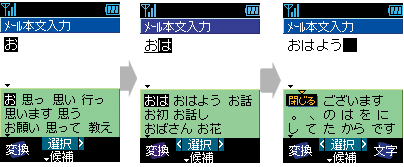
\includegraphics[width=9cm,bb=0 0 404 600]{figures/ac2b347a7042f920edd576ee07c4b7f4.png}
  \caption{POBox.}
  \label{example1}
\end{figure}

コンピュータが人間の操作を予測することにより
人間の負担を減らす「予測インタフェース」システムの研究が従来から行なわれていましたが、
POBoxはこれをテキスト入力に応用したものです。
%
予測型入力システムは、携帯電話のような小型のモバイル機器での
テキスト入力に便利だということが評価され、
現在の携帯機器でのテキスト入力手法の標準となっています。

テキスト入力に予測インタフェースを利用するという手法は、
障害者向けの入力インタフェースとして従来から利用されていましたが、
POBoxは、誰もが使えるユニバーサルなインタフェースとしてデザインされているところが重要です。
ユニバーサルなユーザインタフェースの工夫によって
あらゆる人々が使えるシステムを作ることが可能になることを示せた点は意義があったと考えています。

現在、予測型テキスト入力手法は
各種スマホの入力手法や
障害者用入力システム\footnote{
https://www.ideafront.jp/PeteHP/
}
などに幅広く利用されています。

\begin{figure}[!]
  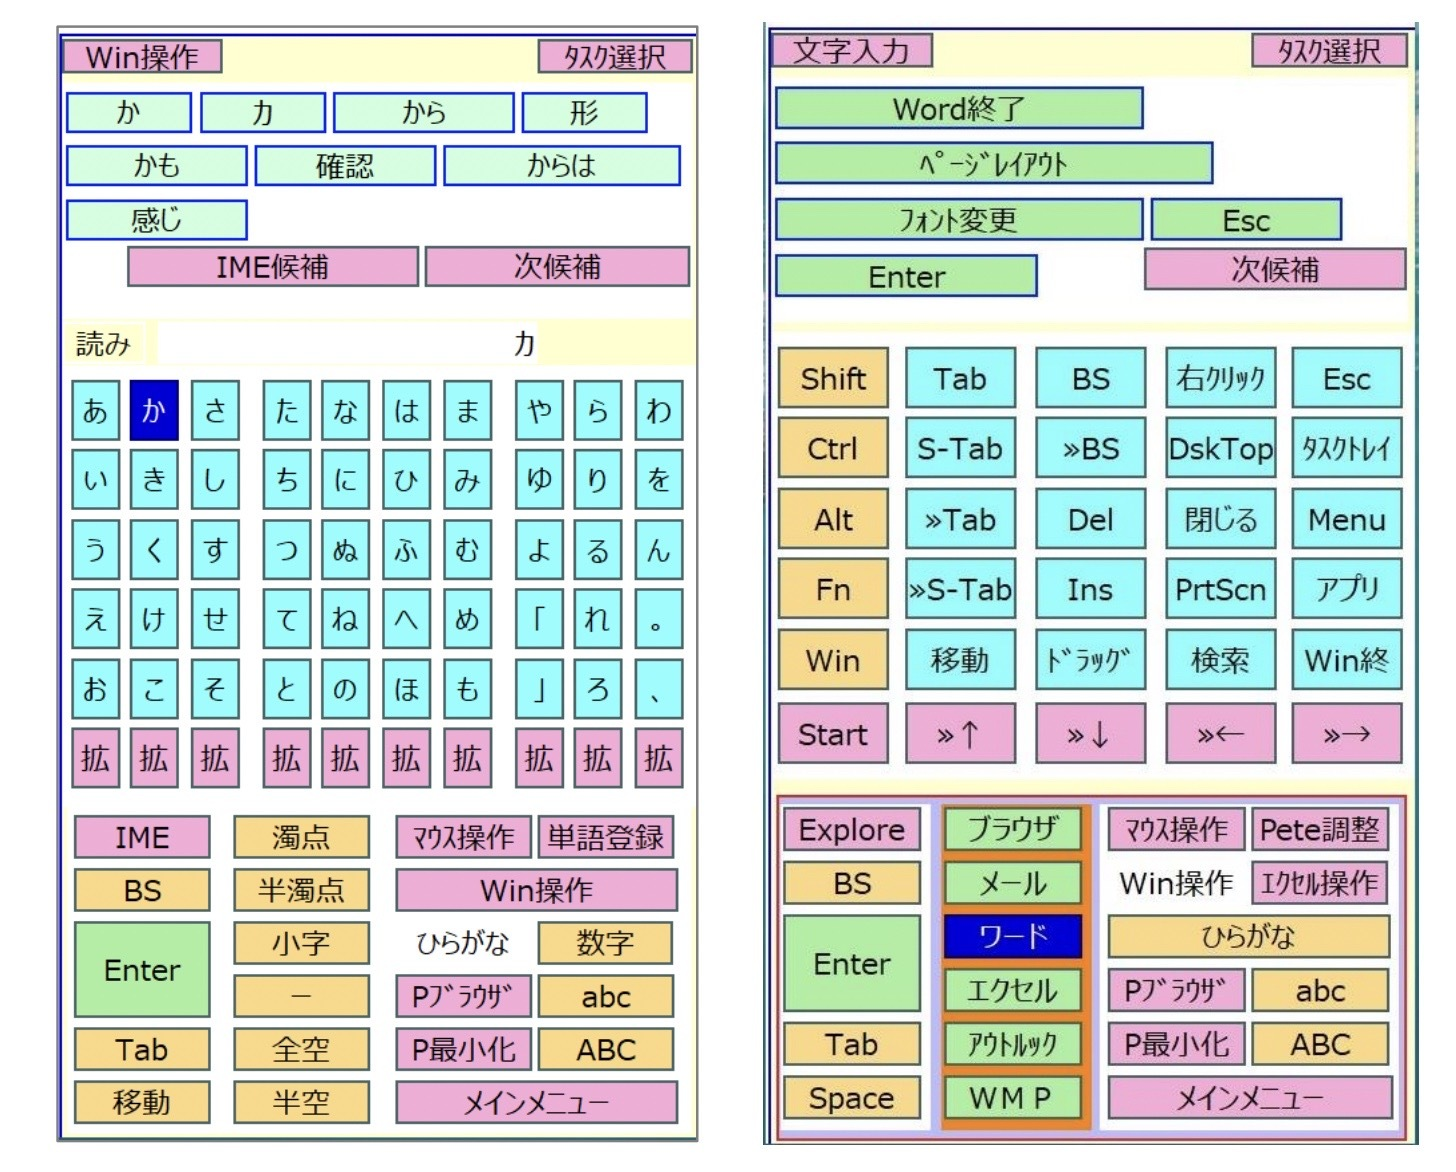
\includegraphics[width=9cm,bb=0 0 1456 1172]{figures/a2f652e2f488b96974e92f8198f49469.jpg}
  \caption{PETE.}
  \label{example1}
\end{figure}



\subsection{思考支援}

アイデアをまとめたり文章を書いたりするのは難しい作業です。
ワープロ、{\TeX}、HTMLなどを使って綺麗な文章を作ることはできますし、
アイデアや考えをまとめるためのシステムやサービスが近年多数提案されていますが、
決定版といえるものはまだ無いかもしれません。

頭の中の考えをまとめたいときや
情報を共有したいとき、
「Wiki」を使うと効果的だと考え、
Gyazz\cite{gyazz}というシステムを作成して長年利用してきました。
現在「Scrapbox」\footnote{scrapbox}という名前で商品化しています。
Scrapboxでは、
ブラウザを使ってネットで手軽情報を書いたり共有することができます。
またページ間のリンクを簡単に作ることができるので、
様々な用途に使うことができます。

\begin{figure}[t]
  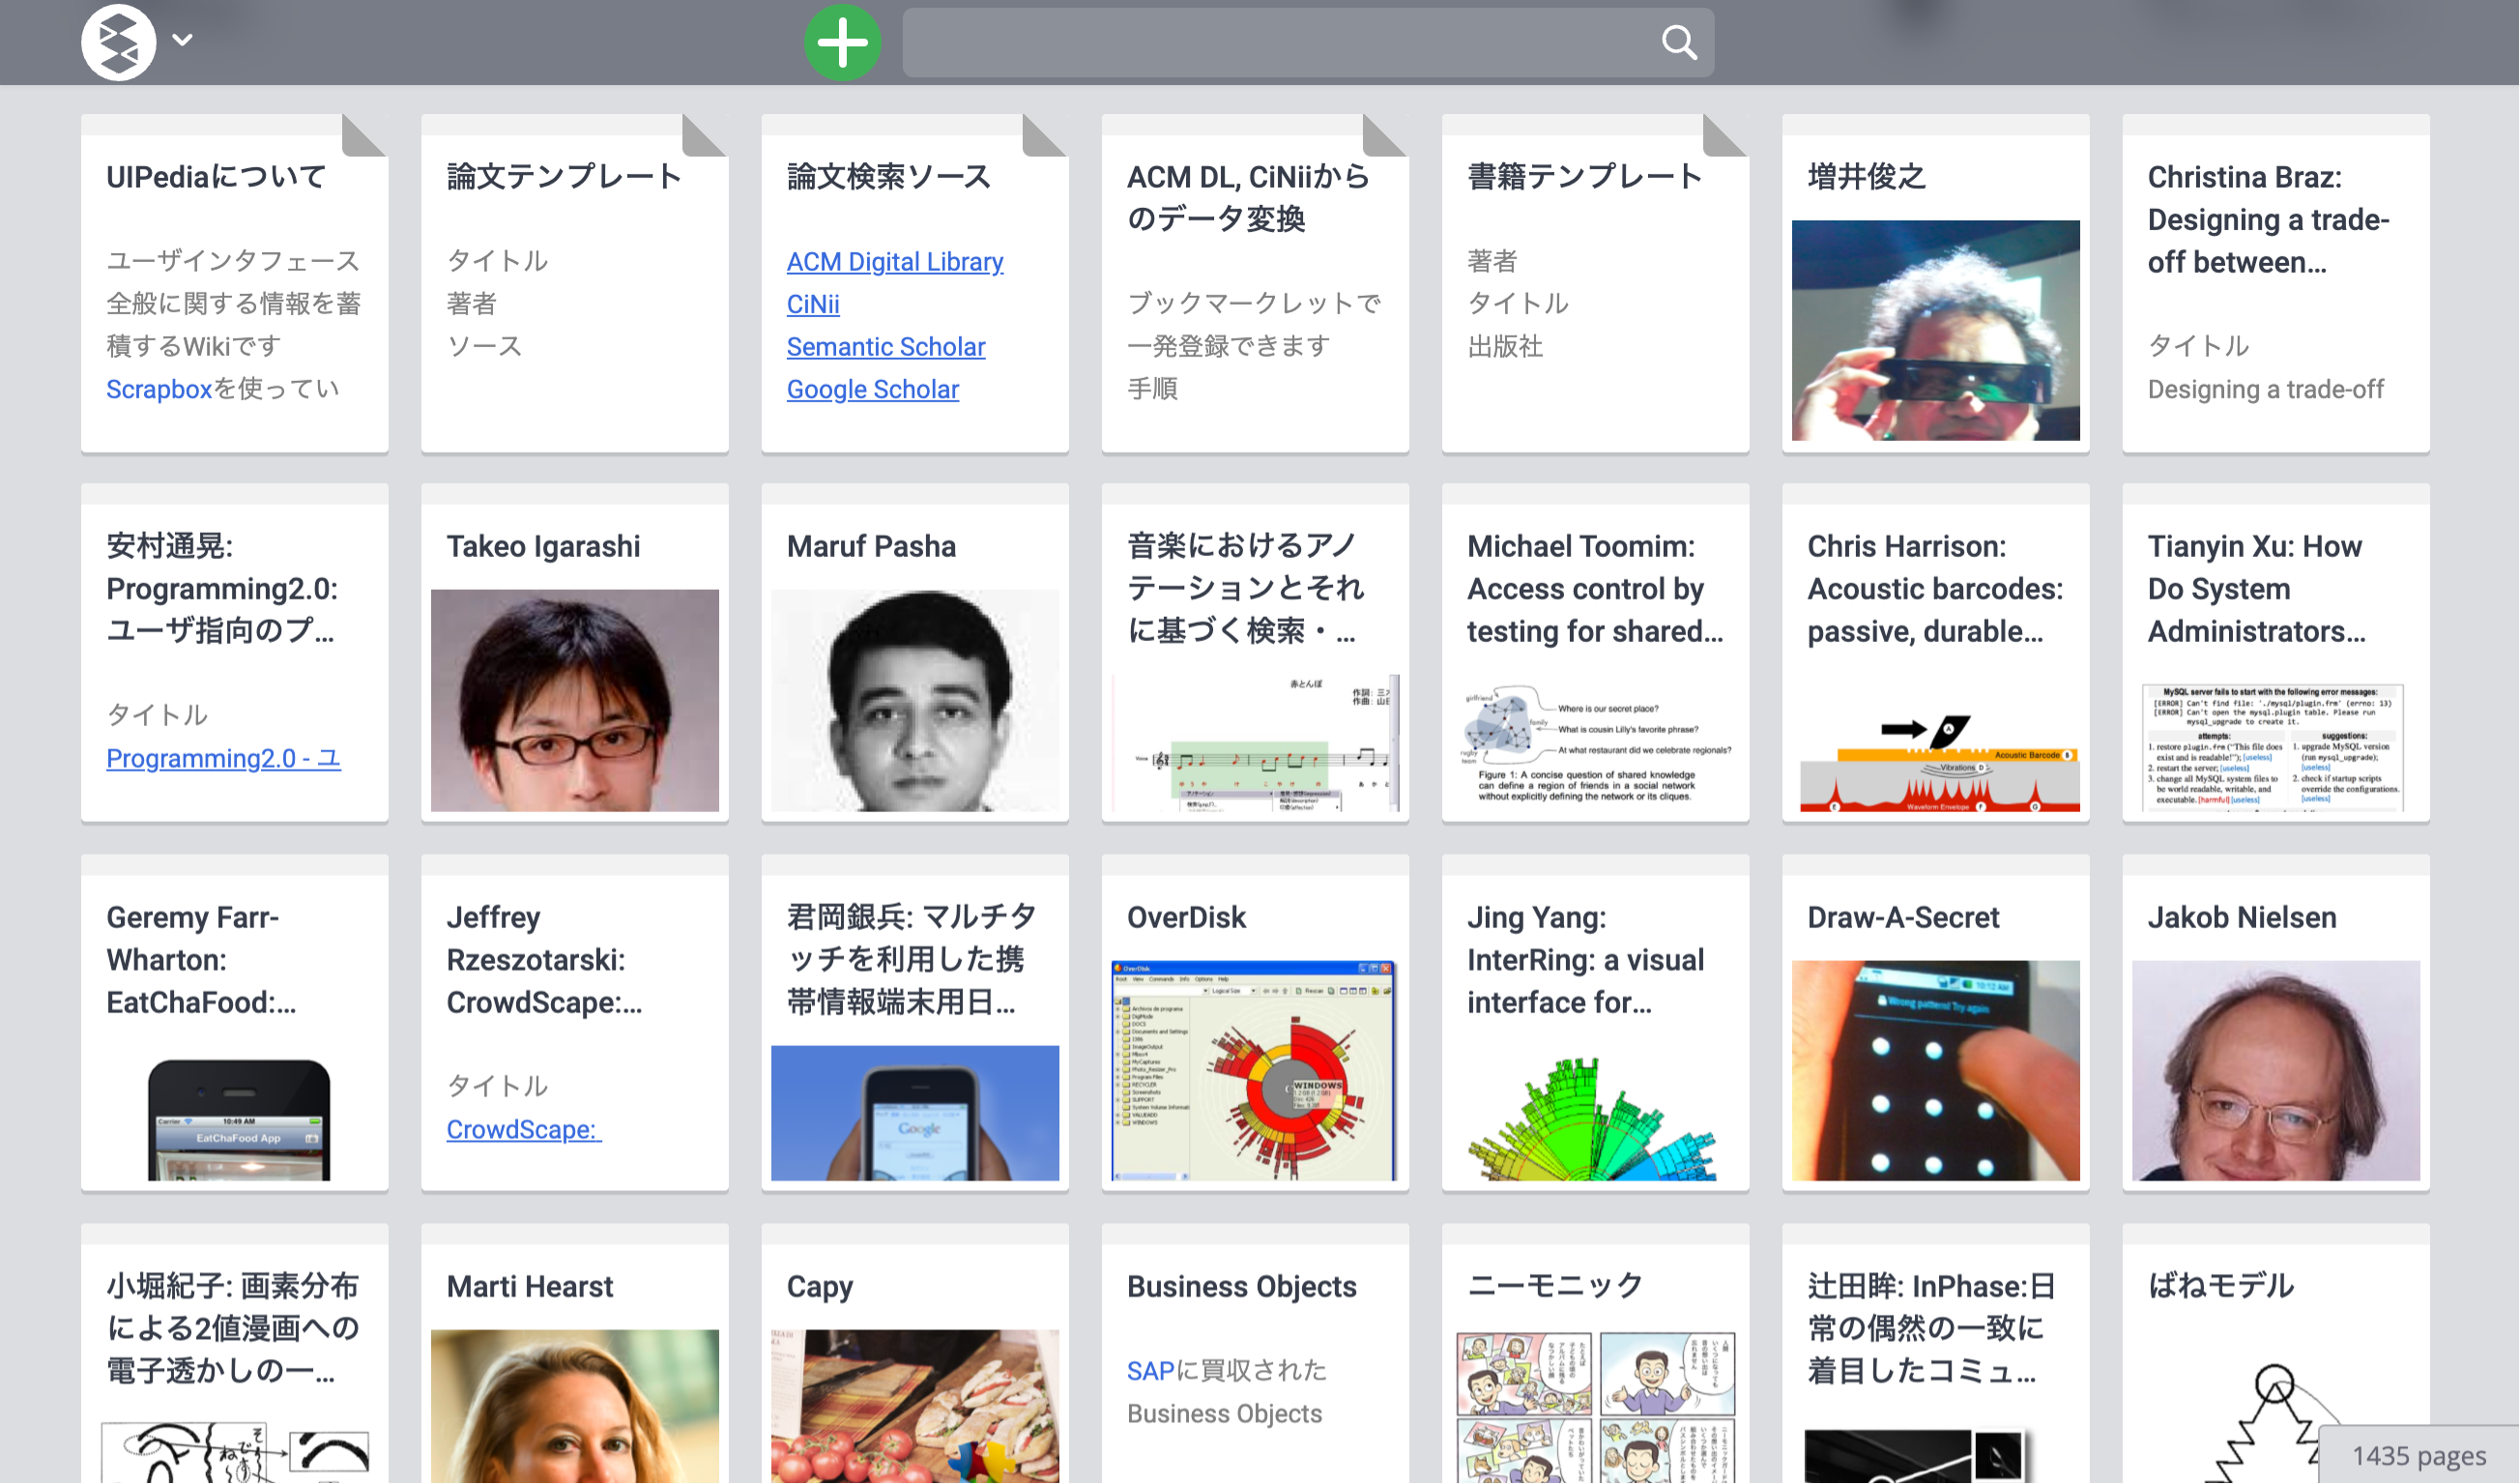
\includegraphics[width=9cm,bb=0 0 2607 1535]{figures/13982c755fdc0c60af2548c0a6589543.png}
  \caption{Scrapboxを使った情報整理}
  \label{example1}
\end{figure}

\begin{figure}[t]
  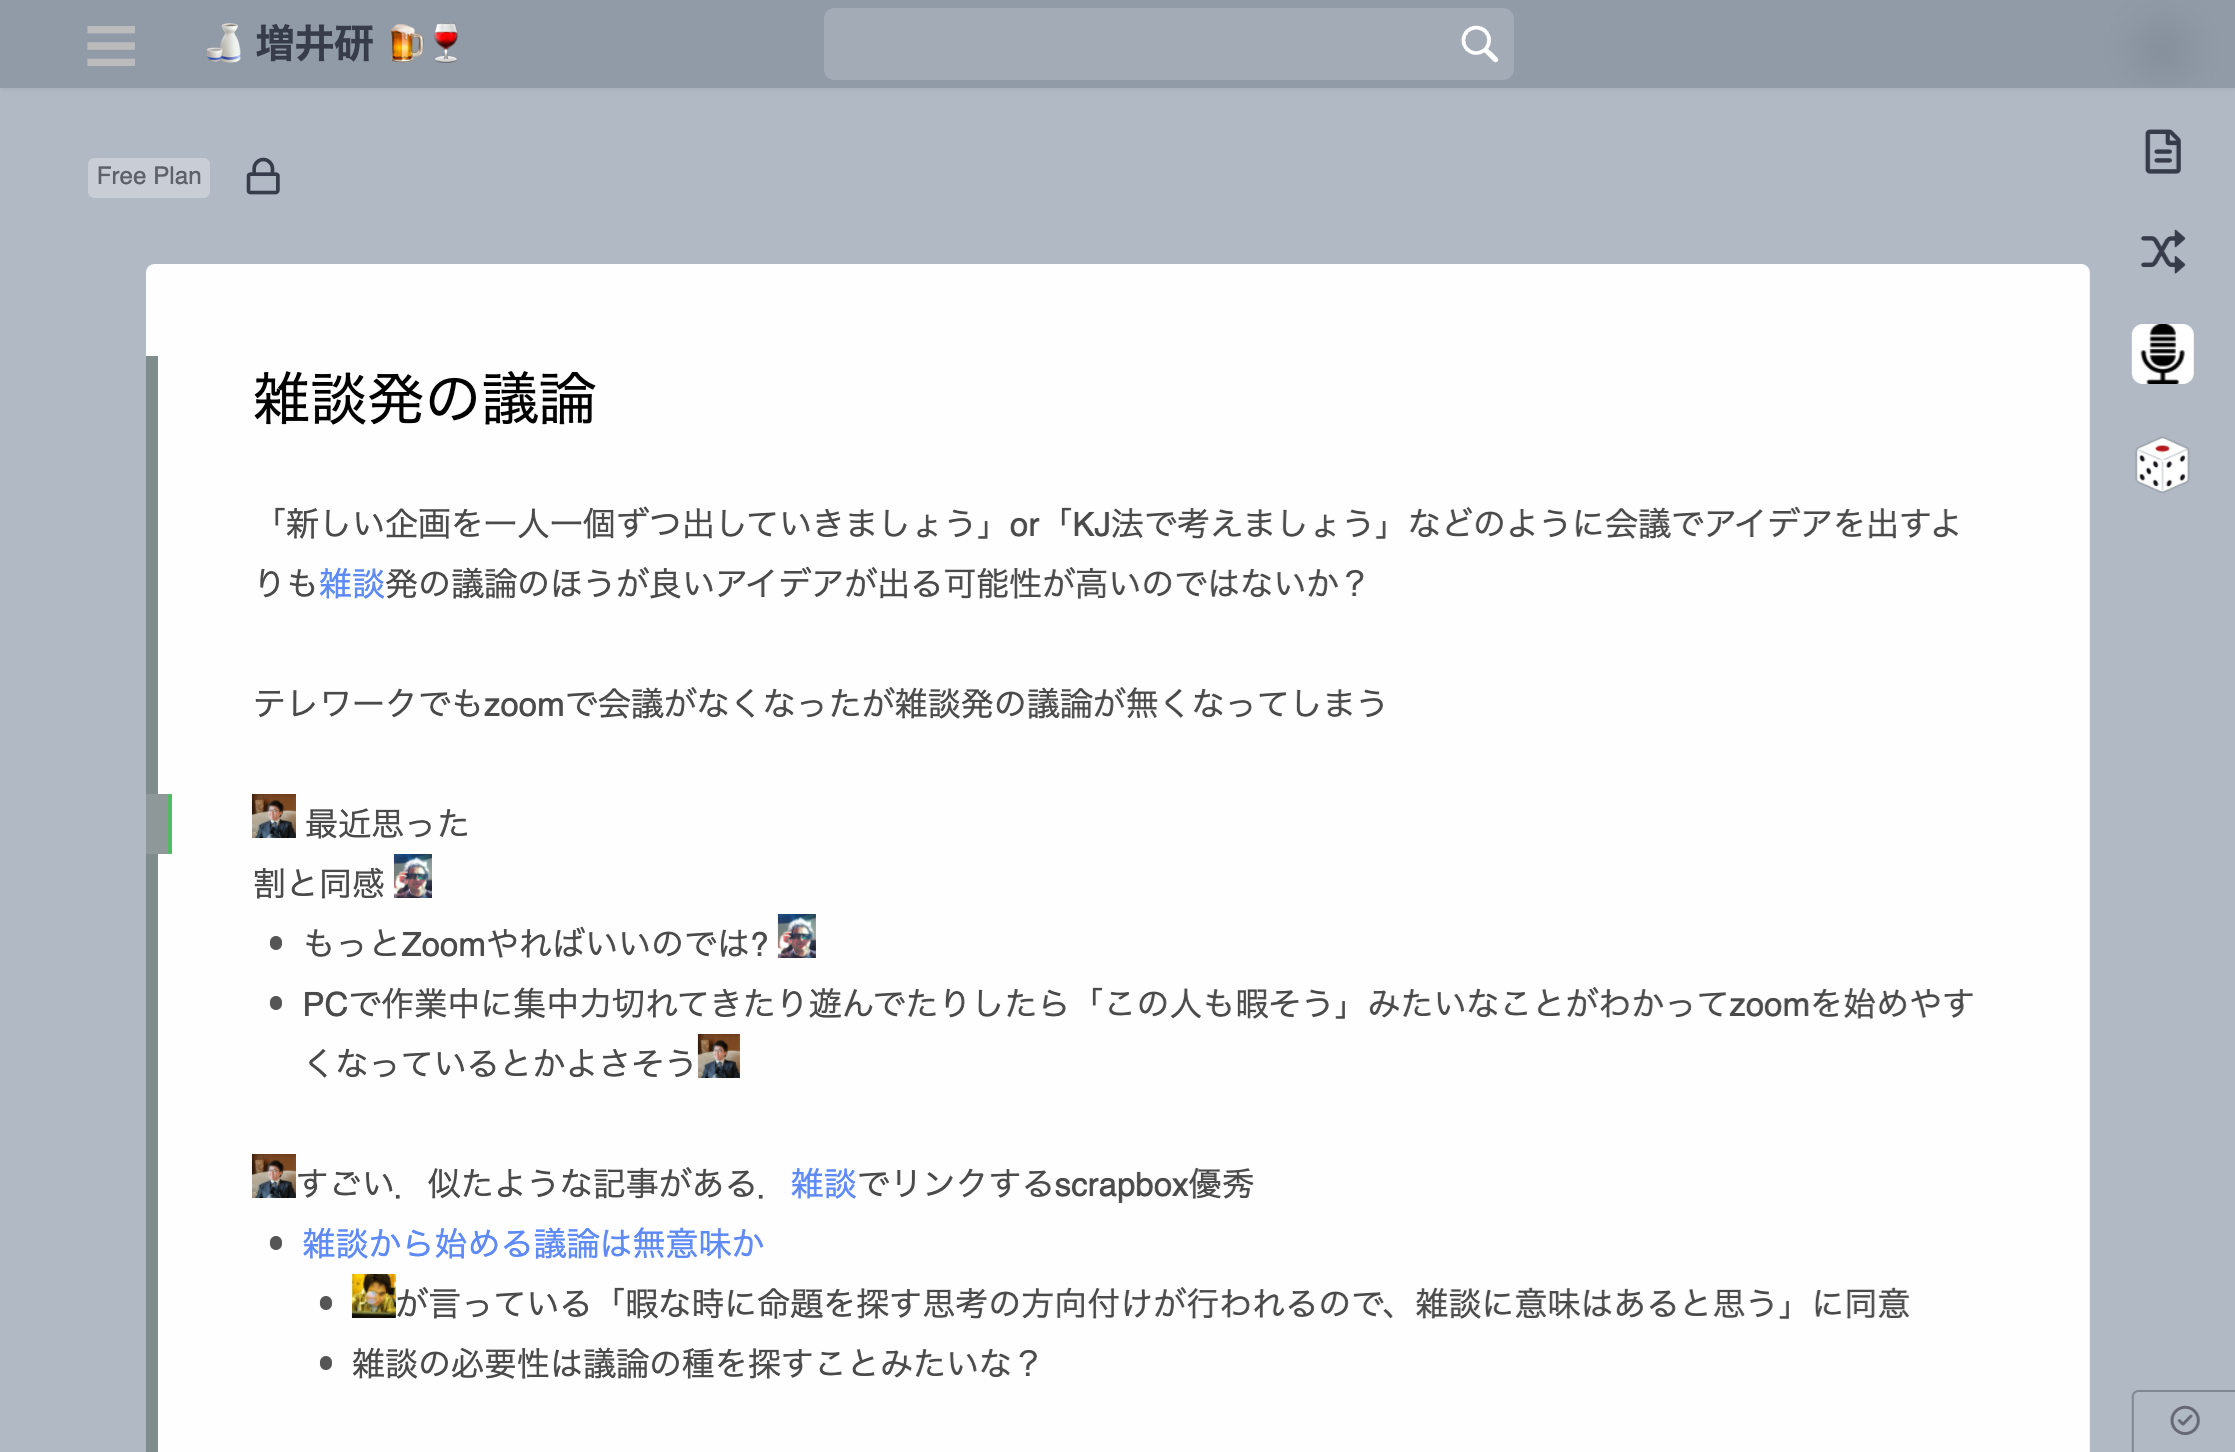
\includegraphics[width=9cm,bb=0 0 2235 1452]{figures/cca2e0eaed298ea4952a26d2effa238c.png}
  \caption{Scrapboxを使った情報整理}
  \label{example1}
\end{figure}


\subsection{検索支援}

複雑なシステムやサービスが身のまわりに増えてきていますが、
使い方などがわからないとき問題を解決する方法はまだまだ不充分です。
パソコンOSやアプリにはヘルプ機能が標準されていますが、
ヘルプシステムを使って問題が解決できることは少ないので、
ほとんど使われていないようです。
今のところ、Google検索したり他人に聞いたりすることで問題を解決してることがほとんどです。

\begin{figure}[t]
  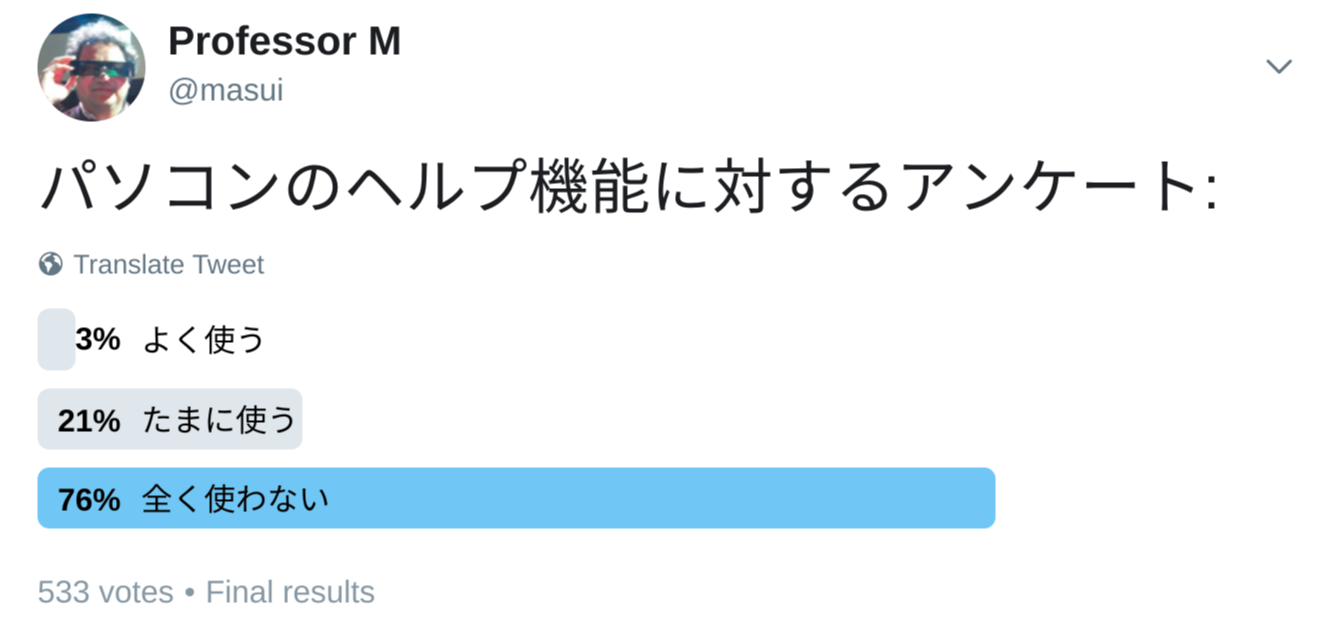
\includegraphics[width=9cm,bb=0 0 1332 623]{figures/383ee54c265ebbb88778d7ea0fbea5b1.png}
  \caption{Helpは使われている?}
  \label{example1}
\end{figure}

% 2019年2月28日 2:24

情報検索はキーワード検索を使うことが多いですが、
ユーザの頭の中の悩みを表現する単語とヘルプ文書のテキストが違っている場合、
必要な情報をうまくみつけるのは困難です。

このような問題を解決するため、
頭の中に出現しそうなキーワードにマッチするあらゆるヘルプ文書を用意しておき、
キーワードと曖昧検索を行なうことによりヘルプを実現する「展開ヘルプ」\cite{xxx}技術を開発し、
「Helpfeel」という商品名でサービスをしています。

\subsection{コンテンツ閲覧}

最近のネットには大量のコンテンツが存在し、
パソコンやテレビでそれらを楽しむことができますが、
コンテンツを選択するための操作は難しいのが普通です。

ふたつのキーだけを利用して大量のコンテンツを選択して楽しむことができる
「Serencast」システムを開発しました\cite{seren}。
Serencastを利用すると、
複雑なリモコン操作を全くせずに大量のコンテンツをブラウジングできます。

\begin{figure}[t]
  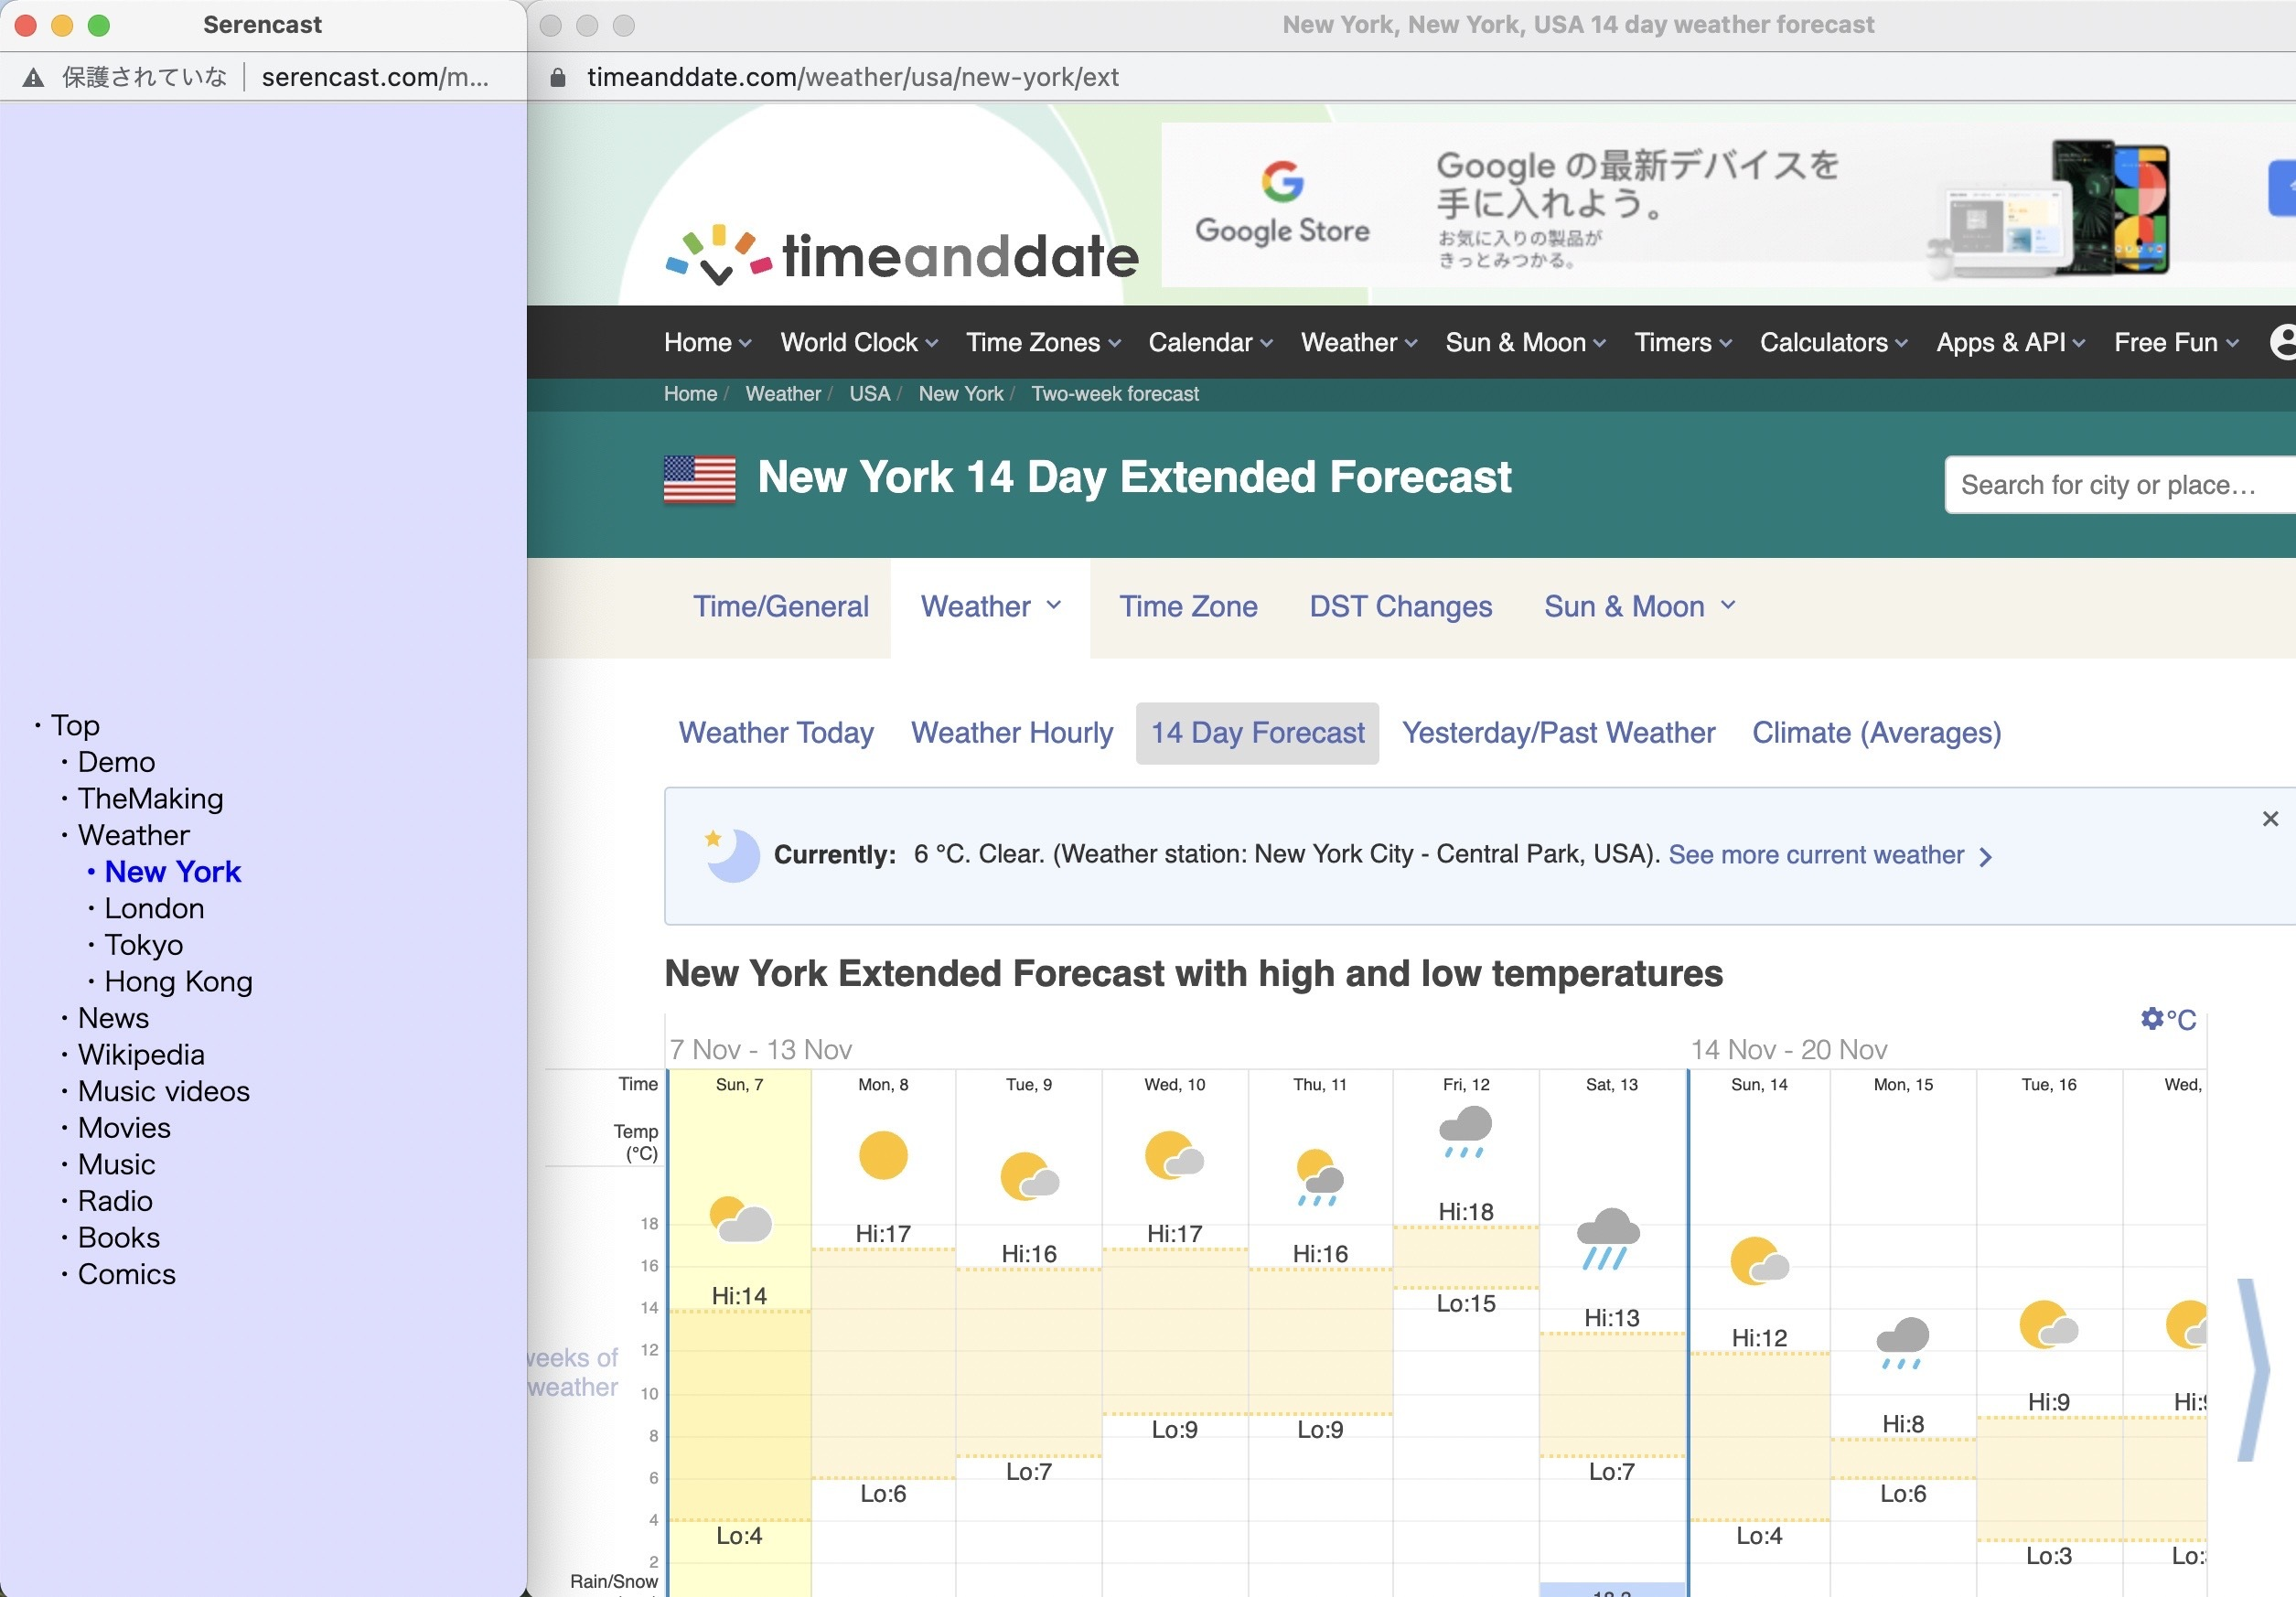
\includegraphics[width=9cm,bb=0 0 2510 1746]{figures/bb4027e2e210bc16450f0120a2987458.jpg}
  \caption{Serencast}
  \label{example1}
\end{figure}

\subsection{パスワード管理}

ネット上のサービスを利用するとき
サービスごとに異なるIDやパスワードが必要になることが多く、
パスワードの管理が大変になってきています。
従来はパスワードは人間の頭で覚えることになっていましたが、
サービスの種類だけパスワードを覚えることは不可能になっています。
異なるサービスで同じパスワードを利用することは危険なので、...

沢山のパスワードを利用するためには
「パスワード管理システム」が広く利用されています。
しかし、パスワード管理システムを利用するためにパスワードが必要ですし、
特殊なアプリケーションはどこでも使えるとは限りません。

こういう問題を解決するために、
既に自分が覚えているエピソード記憶からパスワードを生成して利用できる
「EpisoPass」というシステムを開発しました。
自分だけが覚えているエピソード記憶を利用して...

\section{まとめ}

長年にわたり、誰もがいつでもどこでも利用できる
ユニバーサルなアプリケーションやサービスの開発に勤めてきました。
有用なアプリケーションを作成するためには
基礎的なコンピュータサイエンスの技術が必要です。

\chosha{増井俊之}{
  1984年東京大学大学院工学系研究科電子工学専門課程修士課程修了。 工学博士。
  シャープ、ソニーコンピュータサイエンス研究所、産業技術総合研究所、Apple Inc.などに勤務後、
  2009年4月より慶應義塾大学]環境情報学部教授。
  情報検索、テキスト入力、情報視覚化、実世界指向インタフェース、予測インタフェース、認証技術など、
  ユーザインタフェースに関連する幅広い研究開発を行なっている。
  携帯電話やスマートフォンで広く利用されている予測入力システムPOBoxや
  フリック入力システムの開発者。
  Gyazo, Scrapbox, Helpfeel, EpisoPass, 本棚.orgなど
  各種のWebサービスを運用中。
  WISSの話も書く
  }
  

\end{document}

% https://scrapbox.io/masui/%E3%82%BD%E3%83%95%E3%83%88%E3%82%A6%E3%82%A7%E3%82%A2%E7%A7%91%E5%AD%A6%E4%BC%9A_%E5%9F%BA%E7%A4%8E%E7%A0%94%E7%A9%B6%E8%B3%9E%E8%AC%9B%E6%BC%94
